\chapter{Performance Profiles}
These experiments were last updated at February 8, 2022.

Let $Q$ and $k$ denote respectively the CVRP vehicle capacity and number of vehicles.
Define a scale factor $s \in \N$, a new CVRP instance is generated from the old one using the following steps (described as pseudoalgorithm):

\begin{align}
	Q \gets Q \times s \\
	k \gets \ceil*{\frac{k}{s}}
\end{align}

Each performance profile follows the syntax:

\begin{verbatim}
	<FAMILY-NAME>-scaled-<s>-last-10
\end{verbatim}

where \texttt{<FAMILY>} denotes the CVRP instances family (i.e. E, F, etc) and \texttt{<s>} is the scale factor for the vehicle capacity.
The term \texttt{last-10} is used to denote that the performance profile uses only the last 10 pricing iterations for performing the comparison.

At the time of writing, only the following scaling factors were tested: $s = 1.0,\ s = 2.0,\ s = 4.0$.

\newcommand{\IncludePerfProf}[1]{
	\begin{figure}[ht]
		\centering
		\begin{subfigure}{0.5\textwidth}
			\centering
			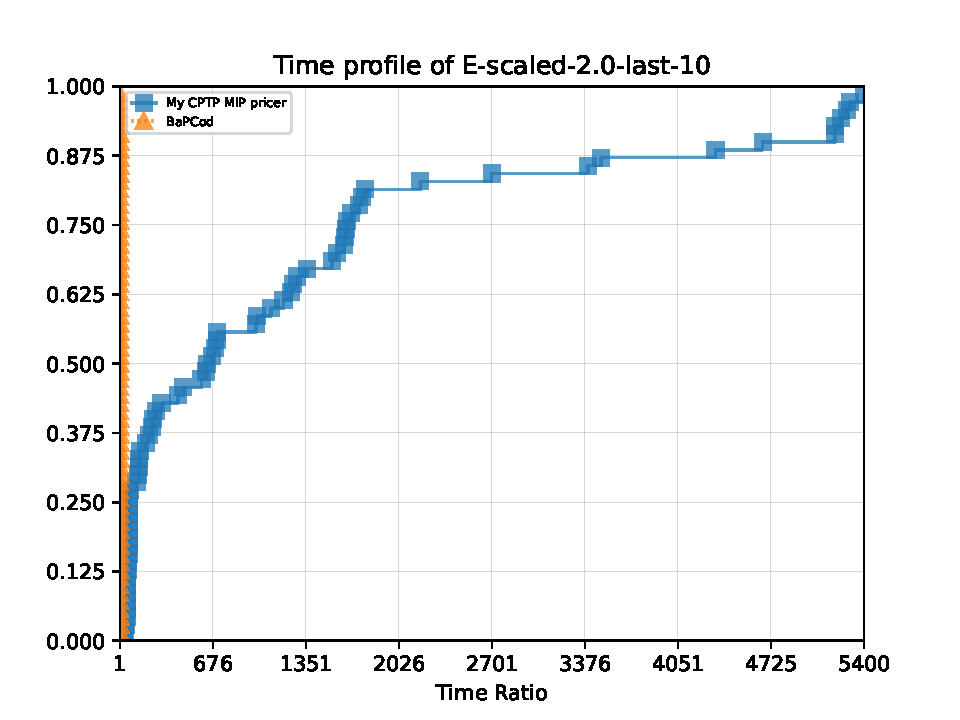
\includegraphics[width=1.0\linewidth]{#1/TimeRatioPlot.pdf}
		\end{subfigure}%
		\begin{subfigure}{0.5\textwidth}
			\centering
			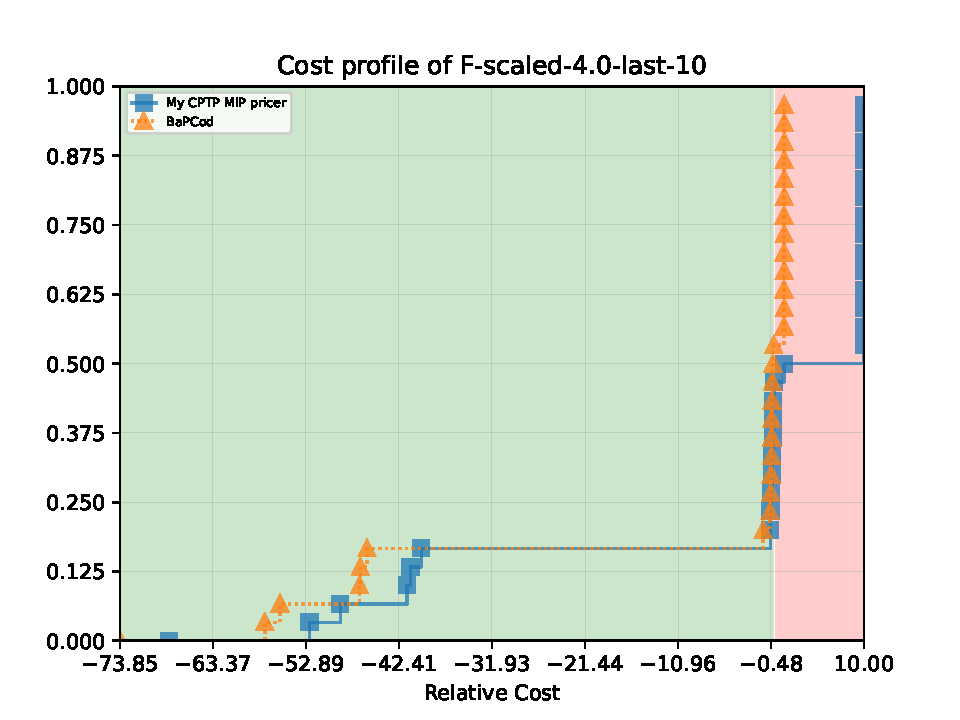
\includegraphics[width=1.0\linewidth]{#1/RelativeCostPlot.pdf}
		\end{subfigure}%
	\end{figure}
}

\forcsvlist{\IncludePerfProf}{
	Imgs/perfprofs/E-scaled-1.0-last-10,
	Imgs/perfprofs/E-scaled-2.0-last-10,
	Imgs/perfprofs/E-scaled-4.0-last-10,
	Imgs/perfprofs/F-scaled-1.0-last-10,
	Imgs/perfprofs/F-scaled-2.0-last-10,
	Imgs/perfprofs/F-scaled-4.0-last-10,
}
